% Load float before the class loads hyperref, avoiding duplicate float anchors.
\RequirePackage{float}
\documentclass[a4paper,fleqn]{cas-sc}

\usepackage[authoryear]{natbib}
\usepackage{amsmath,amssymb}
\usepackage{booktabs}
\usepackage{threeparttable}
\usepackage{graphicx}
\usepackage{multirow}
\usepackage{lineno}
\usepackage[section]{placeins}
\usepackage{xcolor}
\usepackage{setspace}
\usepackage{amsmath}

\ExplSyntaxOn
\cs_new_eq:NN \lr_cusum_original_make_tbl_caption:nn \__make_tbl_caption:nn
\cs_set:Npn \__make_tbl_caption:nn #1#2
  {
    \group_begin:
      \skip_set:Nn \l_tbl_abovecap_skip {3pt}
      \setstretch{1.5}
      \lr_cusum_original_make_tbl_caption:nn {#1} {#2}
    \group_end:
  }
\cs_new_eq:NN \lr_cusum_original_make_fig_caption:nn \__make_fig_caption:nn
\cs_set:Npn \__make_fig_caption:nn #1#2
  {
    \group_begin:
      \skip_set:Nn \l_fig_abovecap_skip {3pt}
      \setstretch{1.5}
      \lr_cusum_original_make_fig_caption:nn {#1} {#2}
    \group_end:
  }
\ExplSyntaxOff

\begin{document}
\linenumbers

\let\WriteBookmarks\relax
\def\floatpagepagefraction{1}
\def\textpagefraction{.001}

\shorttitle{Mapping recurrent harvests in Ecuadorian balsa plantations}
\shortauthors{Rao et al.}

% TODO(author): Confirm corresponding-author marks and email assignments before submission.
\author[1]{Keyi Rao}[orcid=0000-0001-8443-9819]\cormark[1]
\credit{Conceptualization, Methodology, Software, Visualization, Data curation, Formal analysis, Project administration, Writing -- original draft}

\author[1]{Shixin Dong}[orcid=0009-0005-7299-5312]\cormark[1]
\credit{Methodology, Software, Visualization, Validation, Writing -- original draft}

\author[2]{Zhongwen Hu}[orcid=0000-0003-2689-3196]
\credit{Validation, Funding acquisition, Writing -- review and editing}

\author[3,4]{Cesar Ivan Alvarez}[orcid=0000-0001-5629-0893]
\credit{Conceptualization, Methodology, Writing -- review and editing}

\author[5]{Yuanyong Dian}[orcid=0000-0002-4957-3681]
\credit{Validation, Writing -- review \& editing}

\author[1]{Zhaocong Wu}[orcid=0000-0003-2435-5538]
\ead{zcwoo@whu.edu.cn}
\credit{Conceptualization, Supervision, Funding acquisition}

\affiliation[1]{organization={School of Remote Sensing and Information Engineering, Wuhan University},
  addressline={No. 299 Bayi Road, Wuchang District}, city={Wuhan}, postcode={430072},
  state={Hubei}, country={China}}
\affiliation[2]{organization={School of Architecture and Urban Planning and MNR Key Laboratory for Geo-Environmental Monitoring of Great Bay Area, Shenzhen University},
  addressline={No. 3688 Nanhai Avenue, Nanshan District}, city={Shenzhen},
  postcode={518060}, state={Guangdong}, country={China}}
\affiliation[3]{
    organization={College of Horticulture \& Forestry Sciences, 
    Huazhong Agricultural University},
    addressline={No. 1 Shizishan Street, Hongshan District},
    city={Wuhan},
    postcode={430070},
    state={Hubei},
    country={China}
}
\affiliation[4]{organization={Institute of Geography, Faculty of Applied Informatics, University of Augsburg},
  addressline={Universit\"atsstra\ss e 12}, city={Augsburg}, postcode={86159}, country={Germany}}
\affiliation[5]{organization={Maestr\'ia en Sistemas de Informaci\'on Geogr\'afica, Topograf\'ia Automatizada y Fotogrametr\'ia Digital, Universidad Cat\'olica de Santiago de Guayaquil},
  city={Guayaquil}, country={Ecuador}}
  
\cortext[cor1]{Corresponding author}

% Detecting 突出识别事件的过程与能力。标题以它开头，读者首先关注CUSUM如何提取候选、如何排除误检，以及事件日期是否准确。
% Mapping 突出带有空间位置的事件及其属性产品。标题以它开头，读者首先关注哪些地点何时发生采伐、哪些地点发生多次，以及次数和间隔怎样分布。
% 用 successive，重点是2018—2021、2021—2025这两对前后相邻的事件。用 recurrent，重点是同一地点在观测期内经历了三次采伐
% \title[mode=title]{SAR-based Windowed CUSUM detects recurrent stand disturbances from decadal Sentinel-1 time series in Ecuadorian balsa plantations}
\title[mode=title]{Mapping recurrent harvests in Ecuadorian balsa plantations from decadal Sentinel-1 time series with Windowed CUSUM}

% \begin{abstract}
% Balsa plantations supply lightweight timber, including material for wind-energy infrastructure, but their rapid turnover is difficult to reconstruct under persistent tropical cloud cover. The expanding Sentinel-1 archive offers repeated observations of disturbance and recovery within the same stands. We developed Windowed CUSUM to connect near-decadal, track-specific radar trajectories to recurrent stand-disturbance histories. The framework renews the temporal reference within overlapping windows, separates candidate estimation from central-interval admission, and consolidates directionally and statistically screened detections. Evaluation used 1,093 dated reference events from 462 polygons in 57 spatial blocks. Spatial out-of-fold precision, recall and F1 were 0.789, 0.806 and 0.797, respectively. F1 exceeded the evaluated decrease-filtered ReCuSum implementation by 0.122 (95\% spatial-block bootstrap interval: 0.094--0.149). Component removal identified local-reference windowing as the largest contributor to performance. Temporal truncation nevertheless showed that reliable retrospective dating did not imply immediate detection: recall reached 0.790 with six months of subsequent observations. Application to 3,498 inventory polygons yielded 6,658 detections during 2017--2025 and 3,509 inter-disturbance intervals, with a median of 36 months. Restricting this frozen catalogue to its final five years retained only 1,349 intervals, illustrating the additional historical information available from the longer record rather than an accuracy gain. The framework supports auditable reconstruction of recurrent plantation disturbances, while observation boundaries, incomplete reference histories and uncertain disturbance causes limit interpretation as biological rotation ages.
% \end{abstract}

% Balsa plantations have rapid management turnover, but persistent tropical cloud cover limits optical reconstruction of repeated stand disturbances. 


% Abstract还是主要写方法，增加方法的权重，方法的难度和创新要表达出来。强调 Windowed cusum在几个方面有创新？创新是什么，解决了什么问题，解决应用中的什么问题，不是技术层面的效果
\begin{abstract}
  Short-rotation balsa (\textit{Ochroma pyramidale}) plantations undergo repeated harvest and recovery cycles that are difficult to reconstruct from optical imagery under persistent tropical cloud cover. To address this, we developed \textit{Windowed CUSUM}, a temporally adaptive cumulative-sum framework for recurrent stand-disturbance detection from decadal Sentinel-1 synthetic aperture radar (SAR) time series. The framework addresses three challenges in long-term SAR monitoring. First, burst-level observations are organized into track-specific monthly stand trajectories to maintain consistent acquisition geometry and summarize spatially heterogeneous backscatter. Second, overlapping temporal windows repeatedly renew the local reference, allowing disturbance candidates to be evaluated against the local backscatter context across successive rotations. Third, candidates are screened for negative shifts consistent with canopy loss and for statistical support relative to local background variability. We evaluated the framework using 1,093 visually dated disturbances from 462 balsa stands in Ecuador. Among 1,018 events with paired observations, median VV and VH declines were approximately 1.5~dB despite substantial overlap in absolute backscatter. Under spatial cross-validation, Windowed CUSUM achieved precision 0.789, recall 0.806, and F1 0.797, exceeding decrease-filtered ReCuSum (F1 0.675) and CCDC (F1 0.680). Ablation analysis identified local-reference renewal as the main source of recurrent-event recall, while candidate screening preserved precision. Applied to 3,498 validated balsa plantation polygons during 2017--2025, the framework reconstructed 6,658 disturbances, with a median inter-disturbance interval of 36 months. These results show that decadal SAR trajectories can recover recurrent stand-scale structural disturbances despite heterogeneous backscatter backgrounds, enabling plantation turnover to be reconstructed where optical continuity is limited.
\end{abstract}


% ===================================
% 提出什么方法、解决什么任务；
% 创新一：解决长期背景非平稳；
% 创新二：解决 candidate specificity；
% 数据组织：保证长期观测几何一致；
% 应用结果：36 个月轮伐间隔。

\begin{highlights}
  \item Windowed CUSUM detected recurrent disturbances from decadal Sentinel-1 and achieved F1 0.797
  % Windowed CUSUM 基于十年尺度 Sentinel-1 时序检测反复发生的林分扰动，F1 达到 0.797。

  \item Sliding windows adapt local references to evolving stand backscatter across rotations
  % 滑动时间窗口根据不同轮伐阶段不断变化的林分后向散射状态，自适应更新局部参考。

  \item Candidate screening retains canopy-loss shifts beyond local background variability
  % 候选事件筛选保留与冠层损失一致、且超出局部背景变异的后向散射变化。

  \item Track-specific Sentinel-1 trajectories limit mixing of acquisition geometries
  % 按轨道构建 Sentinel-1 时序轨迹，减少不同观测几何条件的混合。

  \item Balsa disturbance histories showed a median inter-disturbance interval of 36 months
  % 重建的巴沙木扰动历史显示，相邻扰动之间的中位时间间隔为 36 个月。
\end{highlights}

% ===================================
\begin{keywords}
Balsa plantation \sep
Sentinel-1 SAR \sep
forest disturbance monitoring \sep
time-series change detection \sep
CUSUM \sep
plantation rotation
\end{keywords}

\maketitle
\doublespacing

% !TeX root = ../main.tex

\section{Introduction}
\label{sec:introduction}

% 总结全文，为什么要SAR时序监测

Balsa (\textit{Ochroma pyramidale}) is a fast-growing tropical tree species whose wood combines low density with useful mechanical properties, making it valuable for lightweight structures, including wind-turbine blade cores~\citep{Borrega2015Balsa_mechanics,Midgley2010Balsa}. Ecuador is a major source of commercial balsa, and its plantations can undergo management-related turnover on cycles of only a few years under productive tropical conditions~\citep{GonzalezOsorio2010Balsa,CanadasLopez2019BalsaGrowth}. Reconstructing these short-rotation dynamics therefore requires a long and temporally continuous observation record spanning multiple disturbance events within the same stand, rather than a single disturbance label~\citep{Du2022GlobalPlantingYears,Li2022EucalyptusHistory}. This requirement is difficult to meet with optical satellite imagery because persistent cloud cover in tropical Ecuador disrupts temporal continuity and can leave critical disturbance periods unobserved~\citep{DelgadoAguilar2017EcuadorSAR}. Sentinel-1 synthetic aperture radar (SAR) provides a cloud-independent, long-term observation record with frequent repeat acquisitions~\citep{Torres2012S1}, providing the observational basis to investigate whether recurrent stand disturbances can be reliably resolved from long-term SAR trajectories.

% SAR监测的难点

Even with dense SAR observations, reconstructing recurrent stand disturbances remains challenging. Sentinel-1 backscatter responds not only to canopy structure but also to moisture conditions, surface roughness, phenological state, and acquisition geometry, introducing temporal variability that can overlap the signal of structural change~\citep{Reiche2018Bayesian,Doblas2020harmonic,Matthew2021BFAST,vanDerWoude2024S1Disturbance,BorlafMena2023Seasonality}. Seasonality and viewing geometry can alter forest backscatter even in the absence of management change, while the sensitivity of C-band SAR to a given surface-state transition also varies with land-surface conditions~\citep{BorlafMena2023Seasonality,Zhao2021SARExclusion}. Consequently, absolute backscatter does not uniquely identify plantation state across stands and environments. As a stand changes after disturbance and recovery, a fixed historical reference may also cease to represent its current condition~\citep{Li2022EucalyptusHistory,Ygorra2023ReCuSum}. A temporally adaptive reference is therefore central to recurrent disturbance monitoring, allowing persistent structural departures to be distinguished from normal SAR variability.

% literature review

Optical and SAR-based time-series studies have addressed different aspects of forest and plantation change monitoring. Multi-decadal Landsat records have been used to identify successive plantation rotations and quantify productivity~\citep{McMahon2019EucalyptusRotations}, while other optical time-series approaches have reconstructed planting history, harvest timing, generation, rotation length, and stand age in short-rotation plantations~\citep{Du2022GlobalPlantingYears,Li2022EucalyptusHistory}. More recently, month-resolved Landsat--Sentinel observations have improved harvest-date localization and stand-age estimation~\citep{Huang2026EucalyptusAge}. Sentinel-1 studies, in contrast, have focused mainly on disturbance detection and near-real-time monitoring, including Bayesian monitoring, continuous change detection, cumulative sum (CUSUM)-based methods, and coherence-based approaches~\citep{Reiche2018Bayesian,Bullock2022CCDC_S1,RuizRamos2020CUSUMSMC,Ygorra2021CuSum,Akbari2022ClearCut}. Sensitivity to management-related and low-intensity forest disturbances has also been demonstrated~\citep{vanDerWoude2024S1Disturbance,Aquino2022LowIntensity}. Yet reconstructing multiple dated disturbances within the same managed stand from a near-decadal SAR record remains largely unexplored.

% 引出CUSUM方法: 已有 SAR 能检测变化, CUSUM 能积累持续偏离,
% ReCuSum 能处理多变化, CuSum NRT 已经使用滑窗,
% 但仍缺少面向长期林分 recurrent history 的 local-reference 设计

CUSUM methods provide an interpretable way to accumulate persistent departures from a temporal reference~\citep{Page1954CUSUM}. They have been used for continuous forest monitoring and tropical disturbance detection~\citep{RuizRamos2020CUSUMSMC,Ygorra2021CuSum}. ReCuSum extends this principle to multiple disturbances through recursive segmentation~\citep{Ygorra2023ReCuSum}, whereas CuSum NRT applies CUSUM iteratively to short sliding time series to reduce detection delay~\citep{Ygorra2024CuSumNRT}. The remaining challenge in short-rotation plantations is to repeatedly renew the local reference without making later detections contingent on earlier segmentation, while retaining sufficient temporal context to reconstruct a consistent stand-level disturbance history.

% 总结，引出研究内容

We therefore propose \textit{Windowed CUSUM}, which repeatedly renews local references through overlapping temporal windows and retains only negative, statistically supported candidates within each window's central decision interval before consolidating them into recurrent stand-disturbance histories (Fig.~\ref{fig:workflow}). This study aims to (1) characterize the within-stand Sentinel-1 response to historical balsa disturbances; (2) evaluate whether Windowed CUSUM improves recurrent-event detection relative to alternative detectors and remains robust to stand representation, polarization, temporal configuration, and statistical assumptions; and (3) reconstruct recurrent plantation disturbance histories and characterize their spatial and temporal dynamics using stand-level event counts and inter-disturbance intervals.

\begin{figure*}[pos=!htbp]
    \centering
    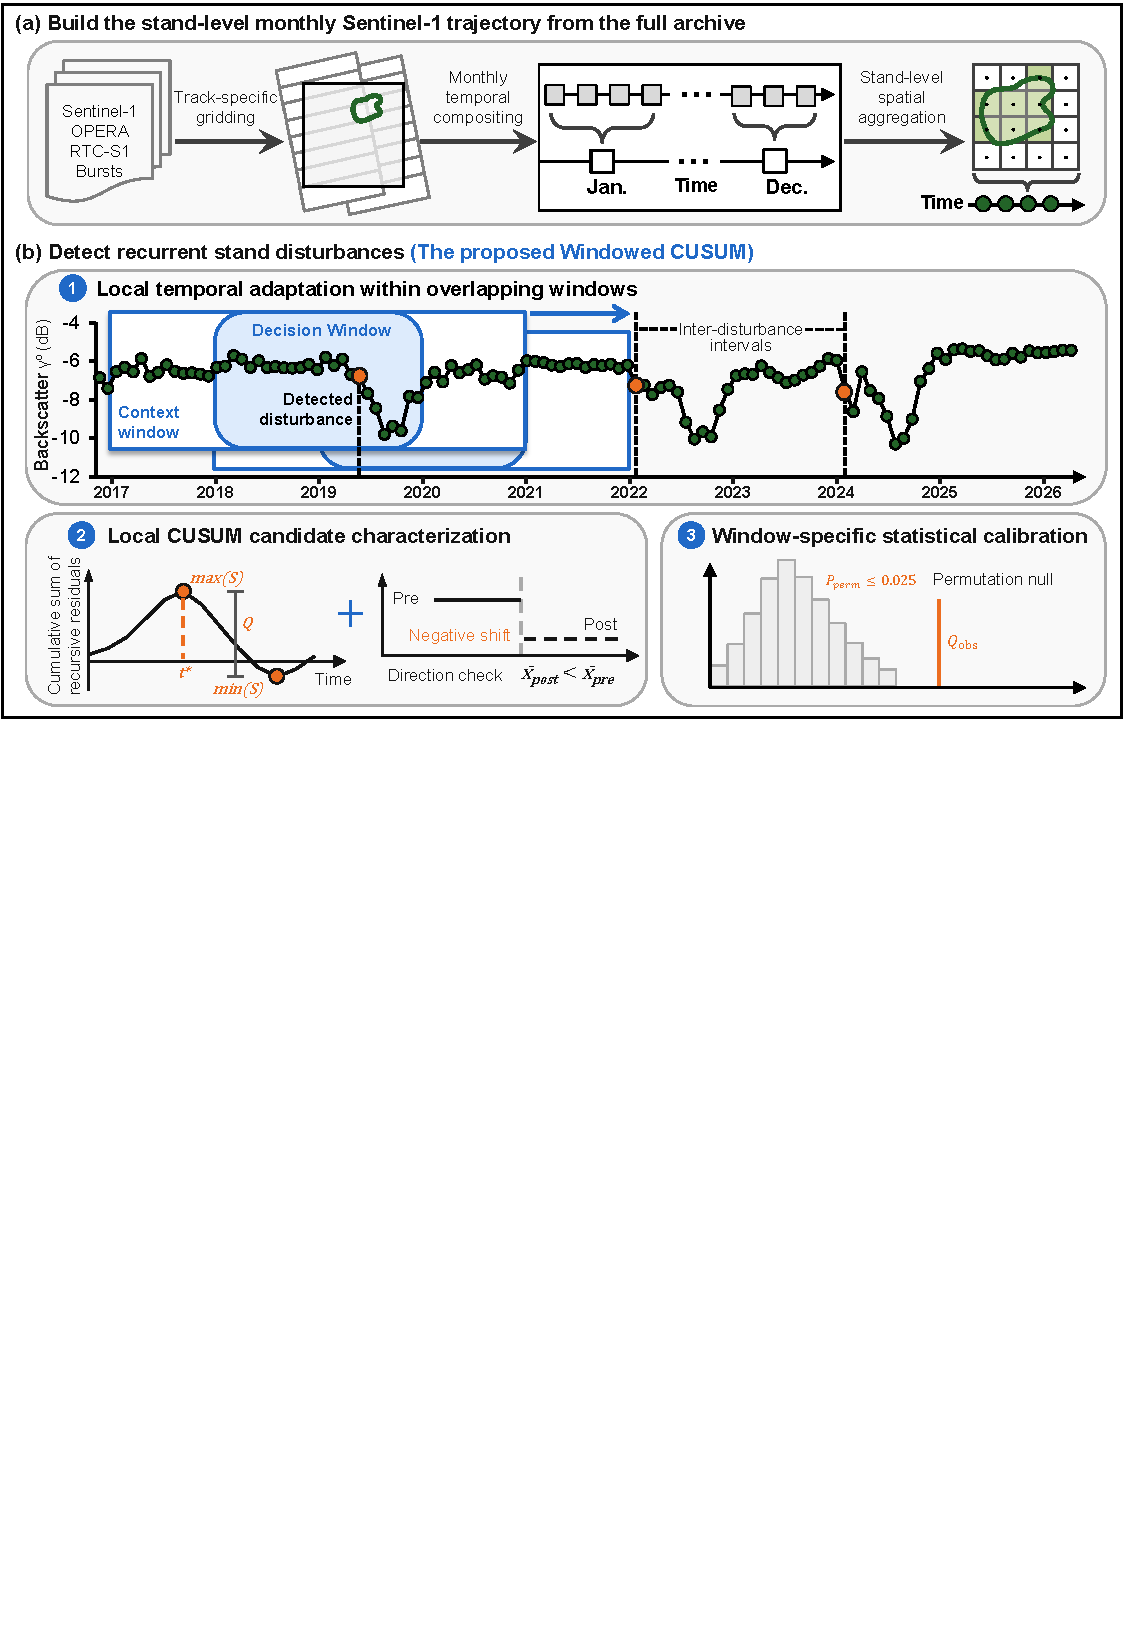
\includegraphics[width=\linewidth]{figures/fig03_workflow.pdf}
    \caption{Conceptual illustration of Windowed CUSUM for one observed balsa stand. (a) Construction of track-specific monthly stand-level Sentinel-1 trajectories. (b) Localization, screening, and consolidation of recurrent disturbance candidates. Within each window, CUSUM identifies candidate magnitude and timing, negative departures are screened against a window-specific permutation null, and accepted candidates are consolidated across overlapping windows.}
    \label{fig:workflow}
\end{figure*}



% !TeX root = ../main.tex
\section{Study region and data}
\subsection{Balsa plantation inventory}

The study covered mainland Ecuador, with particular emphasis on the humid Pacific lowlands and western Andean foothills where commercial BALSA plantations are concentrated as shown in Fig.~\ref{fig:study_area}. Balsa plantation boundaries were obtained from the Ecuadorian Ministry of Agriculture and Livestock through the Geoportal del Agro Ecuatoriano (\url{https://geoportal.agricultura.gob.ec/}).

\begin{figure}[pos=!htbp]
    \centering
    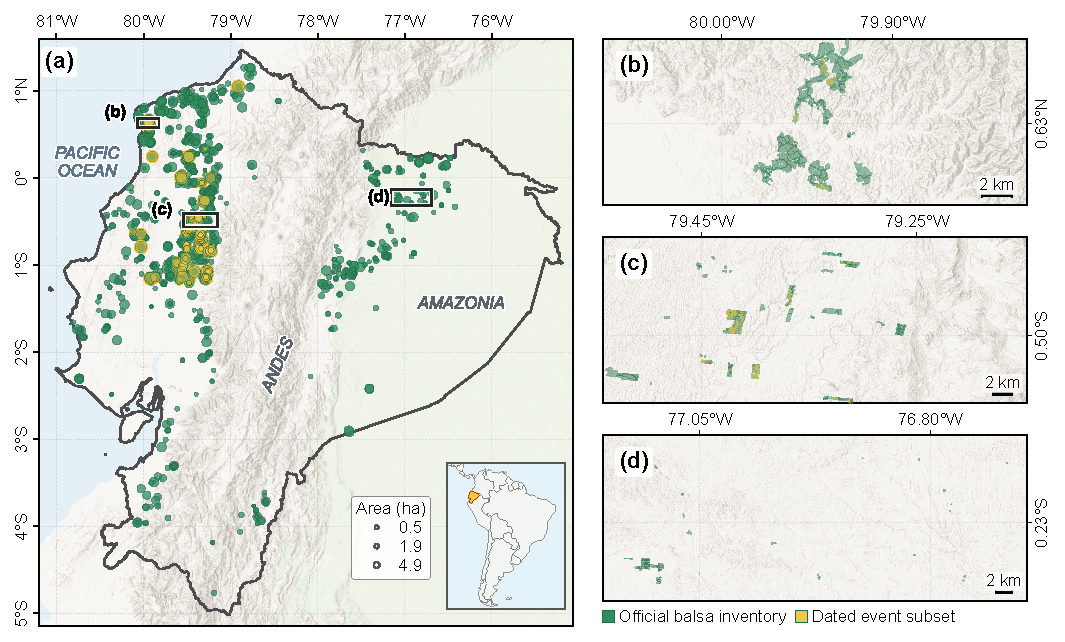
\includegraphics[width=0.92\linewidth]{figures/fig02_study_area.pdf}
    \caption{Study region and official BALSA plantation inventory. Green markers show all 3,890 BALSA polygons, and yellow markers identify the subset containing dated stand-disturbance events. (b)--(d) enlarge representative plantation regions.}
    \label{fig:study_area}
\end{figure}

The source forestry inventory contained 26,206 plantation polygons, of which 3,498 carried the species label BALSA and marked VALIDADO. The validated balsa inventory covered 13,651.85~ha and was divided into three fixed size classes for stratified reporting: small ($\leq1$~ha), medium ($>1$--5~ha), and large ($>5$~ha) (Table~\ref{tab:inventory}).

\begin{table}[pos=!htbp]
    \centering\small
    \caption{Area characteristics of the 3,498 retained BALSA polygons.}
    \label{tab:inventory}
    \begin{tabular}{lrrrrr}
    \toprule
    Area class & Polygons & Count (\%) & Area (ha) & Area (\%) & Median (ha)\\
    \midrule
    Small ($\leq1$ ha) & 1,325 & 37.88 & 497.38 & 3.64 & 0.30\\
    Medium ($>1$--5 ha) & 1,385 & 39.59 & 3,556.10 & 26.05 & 2.33\\
    Large ($>5$ ha) & 788 & 22.53 & 9,598.37 & 70.31 & 8.68\\
    \bottomrule
    \end{tabular}
\end{table}

\subsection{Near-decadal Sentinel-1 observation design}
\label{sec:observation_design}

We used VV and VH backscatter from the OPERA radiometric Sentinel-1 observations were obtained from the NASA OPERA Level-2 Radiometric Terrain Corrected Sentinel-1 (RTC-S1) archive~\citep{shiroma2023OPERARTC,opera2023rtc} and organized using S1-GRiTS v3.0.0 (\url{https://github.com/ottoKae/S1-GRiTS}). OPERA RTC-S1 provides burst-based, radiometrically terrain-corrected $\gamma^{0}$ backscatter at 30-m pixel spacing for VV and VH polarizations.

% 说明组织数据的数量级别
As shown in Table~\ref{tab:s1_observation_coverage}, the Ecuadorian Sentinel-1 SAR archive was organized by four ascending relative-orbit tracks (TK18, TK47, TK91, and TK120). The archive was queried from January 2016 to June 2026, while the first available observations for individual tracks occurred between May and October 2016. In total, 71,134 burst-level RTC products were available, providing dense long-term coverage while preserving track identity throughout subsequent processing.  Detailed acquisition-level compositing, missing-data handling, and stand-level aggregation are described in Section~\ref{sec:s1_timeseries_representation}.

% The 3,498 validated BALSA polygons intersected 40 tile--track combinations, yielding 4,001 polygon--track objects for time-series extraction. Track identity was preserved throughout time-series construction and disturbance detection so that observations from different relative orbits or viewing geometries were not mixed before event consolidation.

\begin{table*}[pos=!htbp]
    \centering
    \small
    \setlength{\tabcolsep}{6pt}
    \caption{Track-specific Sentinel-1 RTC observation coverage used to construct stand-level time series. The archive includes 40 tile--track groups across 31 unique MGRS tiles.}
    \label{tab:s1_observation_coverage}

    \begin{tabular*}{\linewidth}
        {@{\extracolsep{\fill}}lrlrr@{}}
        \toprule
        Track &
        Tile--track groups &
        Observation span &
        RTC burst products &
        stand-level trajectories \\
        \midrule
        TK18  & 19 & Sep. 2016--Jun. 2026     & 36,006 & 3,467 \\
        TK47  & 2  & Jun. 2016--Jun. 2026     & 3,664  & 16    \\
        TK91  & 5  & Oct. 2016--Jun. 2026     & 7,648  & 61    \\
        TK120 & 14 & May. 2016--Jun. 2026     & 23,816 & 457   \\
        \midrule
        Total & 40 & May. 2016--Jun. 2026 &
        \textbf{71,134} & \textbf{4,001} \\
        \bottomrule
    \end{tabular*}
\end{table*}

\subsection{Dated reference events}

Historical disturbance months were assigned by visual interpretation and reconciled to the frozen polygon identifiers. Single-date PlanetScope imagery (approximately 3~m) was the primary evidence source, with monthly Planet basemaps (approximately 4.77~m at the Equator) used where appropriate (Fig~\ref{fig:s1_population_signatures}). Orbit-specific Sentinel-1 observations provided supplementary evidence when cloud cover or incomplete optical observations prevented an unambiguous optical-only date assignment. Interpretation was performed without access to Windowed CUSUM predictions, and ambiguous disturbance dates were not forced into the reference catalogue. After exact polygon--month duplicates were reconciled, the historical catalogue contained 1,093 reference-dated events in 462 validated BALSA polygons distributed across 57 spatial blocks within the 2017--2025 historical evaluation period.
% !TeX root = ../main.tex
\section{Methods}
\label{sec:methods}

% “数据怎么进来、算法怎么评估、消融和 benchmark 怎么做、最后怎样得到 turnover history”；
We developed a workflow to reconstruct recurrent balsa stand disturbances from near-decadal Sentinel-1 observations and translate the detected events into plantation turnover histories (Fig.~\ref{fig:workflow}). The analysis comprised four stages: construction of track-specific stand-level time series, recurrent-event detection with the proposed Windowed CUSUM, spatially structured evaluation and sensitivity analysis, and reconstruction of disturbance recurrence and inter-disturbance intervals. All data preprocessing, detection, evaluation, and statistical analyses were implemented in Python 3.12.

% ====================================================
\subsection{Track-specific Sentinel-1 trajectory construction and stand representation}
\label{sec:s1_timeseries_representation}
% ====================================================

Track-specific monthly Sentinel-1 time series were organized using the Sentinel-1 Gridded Time Series (S1-GRiTS) data-cube framework (\url{https://github.com/ottoKae/S1-GRiTS}). S1-GRiTS preserves pass direction, relative orbit, and polarization as explicit indexing dimensions. For each calendar month $t$, all valid burst-level RTC backscatter observations contributing to the same grid cell, track, and polarization were summarized by their median. The resulting monthly gridded data cube therefore retained separate time series for each track and polarization, with observations from different acquisition geometries kept separate.

% track-specific 不是为了数据管理方便，而是为了让后面的 local-reference assumption 更合理。
As shown in Fig.~\ref{fig:workflow}(a), the monthly grids were subsequently converted to stand-level trajectories using the mapped balsa polygons. For the primary Polygon-first representation, all finite grid-cell values whose centres fell within a polygon were aggregated by their spatial median for each month. We refer to this strategy as Polygon-first because spatial aggregation was performed before disturbance detection. This produced one monthly trajectory for each polygon, track, and polarization. Track identity was retained so that each temporal sequence was constructed under a consistent acquisition geometry, providing an internally comparable temporal background for subsequent local-reference change detection.

Alternative representations were evaluated to determine whether detection performance depended on the spatial aggregation strategy. Polygon-first alternatives included the spatial mean, histogram mode, and a representative grid cell. Pixel-first alternatives retained individual grid-cell trajectories through disturbance detection and subsequently consolidated candidate evidence using connected eight-neighbour support, temporal DBSCAN, or joint space--time DBSCAN~\citep{Ester1996DBSCAN}. Because Pixel-first approaches do not form a single stand trajectory before detection, they require additional spatial-support or clustering parameters, which were selected exclusively from spatial training data as described in Section~\ref{sec:experimental_evaluation}. 


% =====================================================

\subsection{The proposed Windowed CUSUM}
\label{sec:windowed_cusum}

% “这个算法解决什么问题、设计原则是什么、核心模块是什么”。
% 聚焦说明核心设计原则：temporal adaptation + statistical adaptation

Building on the geometry-consistent trajectories described above, Windowed CUSUM was designed to detect recurrent disturbances under temporally heterogeneous Sentinel-1 backgrounds. For such trajectories, disturbance evidence should be interpreted relative to both a dynamically renewed local background and the variability of that background, because backscatter levels and temporal variability can differ among stands and evolve through time. Windowed CUSUM therefore adapts at two levels. Overlapping local-reference windows repeatedly renew the temporal context as each stand evolves, while a window-specific permutation null calibrates each observed CUSUM amplitude against the variability of that same local context. This design avoids reliance on a fixed historical baseline and does not require recursive segmentation after each detected event. Within each window, candidate timing and direction are identified and statistically screened. Accepted candidates are then consolidated across overlapping windows and Sentinel-1 tracks to form a recurrent stand-disturbance history (Fig.~\ref{fig:windowed_cusum_concept}).


\begin{figure*}[pos=!htbp]
    \centering
    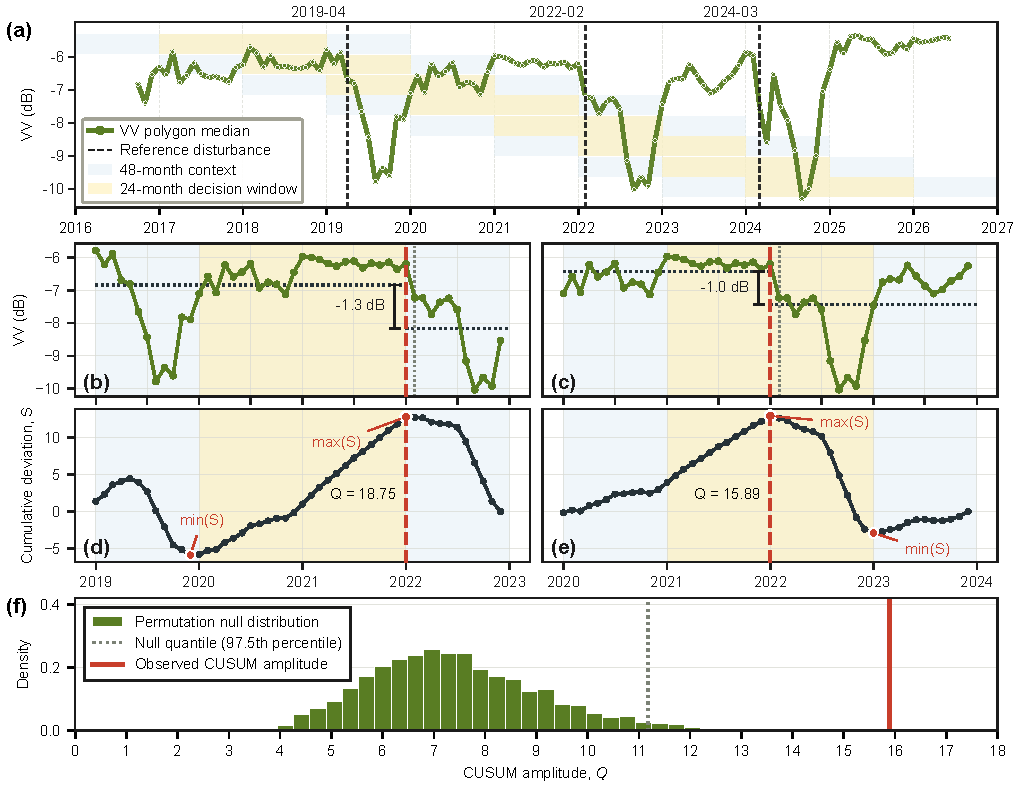
\includegraphics[width=\linewidth]{figures/fig04_windowed_cusum_concept.pdf}
    \caption{Conceptual illustration of Windowed CUSUM for one balsa stand.
    (a) Near-decadal stand-level monthly VV trajectory with reference disturbances and overlapping local-reference windows, showing the temporal context and central decision intervals.
    (b,c) CuSum computation within each window, where candidate points are identified from the maximum cumulative deviation.
    (d,e) Corresponding cumulative-deviation curves, with candidate locations identified from the maximum cumulative residual. The candidate in (d) is rejected because it falls outside the decision interval, whereas that in (e) is retained.
    (f) Evaluation of the retained CUSUM amplitude against its window-specific permutation null.}
    \label{fig:windowed_cusum_concept}
\end{figure*}


% ----------------------------------------------------
\subsubsection{Local temporal adaptation within overlapping windows}
\label{sec:windowed_cusum_windows}
% ----------------------------------------------------
% 当前应该和哪个背景比较？
% 为什么需要局部 temporal reference
% W, S, W_b, D_b
% 为什么 estimation context 和 event admission 分开
% boundary / missing observations / locked W,S

A stand trajectory can contain repeated disturbance and recovery, so a reference defined over the complete record may no longer represent the stand's current condition. Windowed CUSUM therefore evaluates each track-specific trajectory through overlapping local contexts, repeatedly renewing the temporal reference without permanently segmenting the series after an earlier detection. Let $T$ denote the length of the available monthly calendar, $W$ the nominal context-window length, and $S$ the displacement between consecutive windows. For a nominal window beginning at month $b$, the observed context window and its decision window were defined as Equation~\eqref{eq:window_definition}.
\begin{equation}
    \mathcal{W}_b
    =
    [\max(0,b),\,\min(T,b+W)),
    \qquad
    \mathcal{D}_b
    =
    [\max(0,b+S),\,\min(T,b+W-S)),
    \label{eq:window_definition}
\end{equation}
with half-open intervals expressed in calendar months. For interior windows, the central decision window has length $C=W-2S$, requiring $W>2S$.

The two intervals serve different purposes. All finite observations within $\mathcal{W}_b$ contribute to estimation of the local CUSUM, providing temporal context on both sides of a potential transition. Candidate events are admitted only when their estimated month falls within $\mathcal{D}_b$. This central-admission rule reduces sensitivity to transitions estimated near artificial window boundaries, where temporal support is asymmetric. Thus, displacement of $\mathcal{W}_b$ provides temporal adaptation, while $\mathcal{D}_b$ restricts event reporting to the better-supported portion of each local context.

The locked operational configuration used $W=48$ months and $S=12$ months, yielding a 24-month central decision interval for interior windows. Alternative values of $W$ and $S$ were evaluated in the configuration-sensitivity analysis (Section~\ref{sec:experimental_evaluation}). Context windows were clipped to the available record without temporal padding and were subject to the same candidate-admission rules. Each window required at least 12 finite observations, and missing months retained their original calendar positions without interpolation or temporal shifting.

% ----------------------------------------------------
\subsubsection{Local CUSUM candidate characterization}
\label{sec:windowed_cusum_candidate}
% ----------------------------------------------------

Within each local context window, CUSUM was calculated from the finite observations in chronological order. Let $x_1,\ldots,x_n$ denote these observations and $\bar{x}$ their mean. The centred cumulative residual and CUSUM amplitude were defined as Equation~\eqref{eq:local_cusum}, where $n$ is the number of finite observations in the window.
\begin{equation}
    S_t
    =
    \sum_{i=1}^{t}(x_i-\bar{x}),
    \qquad
    Q
    =
    \max_t S_t-\min_t S_t,
    \qquad
    t=1,\ldots,n,
    \label{eq:local_cusum}
\end{equation}
where $S_t$ represents the accumulated departure from the local window mean and $Q$ summarizes the strength of the dominant temporal departure within that window. The window mean serves only as a local centring reference and is not interpreted as an independently known undisturbed-canopy baseline.

For the sustained negative shifts targeted in this study, positive residuals tend to accumulate before the decline and negative residuals afterward, causing the cumulative residual to reach a maximum near the transition between the two states. The candidate location was therefore defined as Equation~\eqref{eq:candidate_position}~\citep{Page1954CUSUM,Ygorra2021CuSum}.
\begin{equation}
    t^*
    =
    \arg\max_t S_t ,
    \label{eq:candidate_position}
\end{equation}
with the first maximum retained in the event of a tie. The index $t^*$ was mapped back to its original calendar month before testing membership in the central decision interval $\mathcal{D}_b$. Candidates outside $\mathcal{D}_b$ were not admitted.

To determine the direction of the candidate change, $x_{t^*}$ was treated as the first post-change observation and the corresponding segment means were
\begin{equation}
    \bar{x}_{\mathrm{pre}}
    =
    \operatorname{mean}(x_1,\ldots,x_{t^*-1}),
    \qquad
    \bar{x}_{\mathrm{post}}
    =
    \operatorname{mean}(x_{t^*},\ldots,x_n).
    \label{eq:time_pre_post_mean}
\end{equation}

Both segments were required to contain at least one finite observation, and only candidates satisfying $\bar{x}_{\mathrm{post}} < \bar{x}_{\mathrm{pre}}$ were retained for statistical calibration. Thus, each local candidate was characterized by its CUSUM amplitude $Q$, candidate month $t^*$, and direction of change. 
% The reported month represents an algorithmic transition boundary at monthly resolution and is not interpreted as the exact physical onset of disturbance.

% ----------------------------------------------------
\subsubsection{Window-specific statistical calibration}
\label{sec:windowed_cusum_permutation}
% ----------------------------------------------------

The raw CUSUM amplitude $Q$ measures the strength of temporal organization within a local window, but its absolute value is not directly comparable across stands or windows. Sentinel-1 background variability can differ with canopy condition, moisture, seasonality, and acquisition geometry~\citep{BorlafMena2023Seasonality,vanDerWoude2024S1Disturbance}. A common threshold on $Q$ could therefore represent very different levels of evidence in a temporally stable stand and in a highly variable stand.

Windowed CUSUM instead calibrates each observed amplitude against a null distribution generated from the same local observations. For each eligible window, the finite observations were randomly reordered while preserving their values and sample size. This procedure retains the local marginal distribution and overall amplitude of backscatter variability while removing its observed temporal ordering. The CUSUM amplitude was then recalculated for each permutation. Let $Q_{\mathrm{obs}}$ denote the observed amplitude and $Q_j^{\mathrm{perm}}$ the amplitude obtained from permutation $j$. For $B$ permutations, the finite-sample-corrected permutation $p$ value was calculated in Equation~\eqref{eq:permutation_pvalue}~\citep{PhipsonSmyth2010Permutation}.
\begin{equation}
    p_{\mathrm{perm}}
    =
    \frac{
    1+\sum_{j=1}^{B}
    \mathbf{1}
    \left\{
    Q_j^{\mathrm{perm}}
    \geq
    Q_{\mathrm{obs}}
    \right\}
    }{B+1},
    \label{eq:permutation_pvalue}
\end{equation}

where $\mathbf{1}\{\cdot\}$ denotes the indicator function. A small $p_{\mathrm{perm}}$ indicates that an amplitude at least as large as $Q_{\mathrm{obs}}$ is rarely reproduced when the same local backscatter values are present but their temporal ordering is removed. Consequently, the same raw $Q$ can receive different statistical support in different windows because its interpretation is conditional on the variability of the corresponding local trajectory.

The initial calibration used $B=3{,}999$ permutations. Candidates with initial $p_{\mathrm{perm}}$ values between 0.015 and 0.035 were recalculated using $B=19{,}999$ permutations to improve Monte Carlo precision near the operational decision threshold. Candidates were statistically supported when $p_{\mathrm{perm}}\leq0.025$. Deterministic candidate-specific random seeds were used to ensure reproducibility.

The permutation $p$ value quantifies candidate-level evidence under the specified within-window randomization null. It is not interpreted as a posterior probability of disturbance or as global false-discovery control across overlapping windows. Independent permutation also removes short-range temporal dependence and therefore assumes exchangeability under the null. Sensitivity to alternative null formulations that preserve temporal dependence was evaluated separately in Section~\ref{sec:experimental_evaluation}.

Futhurmore, candidates passing the directional and statistical screening were still window-level, track-specific nominations. Because overlapping windows could nominate the same transition repeatedly and different Sentinel-1 tracks could localize the same disturbance to adjacent months, accepted candidates were consolidated within each polygon and polarization. Nominations occurring within one month were grouped into the same temporal event cluster; repeated nominations from the same track did not add support. The representative month was selected by the greatest number of supporting distinct tracks, with the earliest month retained under ties. This produced one ordered polygon-level event sequence per polarization. VV and VH remained separate through detection and consolidation, while polarization configurations were evaluated independently in Section~\ref{sec:experimental_evaluation}.


% % ---------------------------------------------------------------
% \subsubsection{Candidate consolidation into recurrent stand histories}
% \label{sec:windowed_cusum_consolidation}
% % ---------------------------------------------------------------

% Candidates passing the directional and statistical screening remained window-level, track-specific nominations rather than unique disturbance events. The same physical disturbance could be nominated repeatedly by overlapping windows, while independent Sentinel-1 tracks could localize that disturbance to adjacent calendar months because of differences in acquisition timing and local temporal context. Accepted candidates were therefore consolidated before constructing polygon-level recurrent disturbance histories.

% Consolidation was performed separately within each polygon and polarization. Candidate nominations occurring within one month of one another were grouped into the same temporal event cluster. Repeated nominations from overlapping windows on the same track did not contribute additional track support. For each cluster, the representative event month was selected as the month supported by the greatest number of distinct Sentinel-1 tracks, with the earliest month retained when distinct-track support was tied.

% This procedure removed repeated window-level nominations and reconciled small timing differences among track-specific detections to produce a single ordered event sequence for each polygon and polarization. VV and VH were processed independently through detection and consolidation, without averaging the two polarization trajectories. The choice of polarization configuration, including VV-only, VH-only, union, and cross-polarization agreement, was evaluated separately in the sensitivity analysis described in Section~\ref{sec:experimental_evaluation}.



\subsection{Disturbance-history reconstruction}
\label{sec:history}

We counted consolidated detections during 2017--2025. For polygon $m$, the ordered consolidated disturbance months were denoted $H_m=(h_{m,1},\ldots,h_{m,n_m})$, where $n_m$ is the number of detected events. Stand-level recurrence was summarized by $n_m$. For stands with at least two events, consecutive inter-disturbance intervals were
\begin{equation}
    R_{m,k}=h_{m,k+1}-h_{m,k},
    \qquad k=1,\ldots,n_m-1.
\end{equation}
Only adjacent detected events were paired, so no interval was constructed across an intermediate event. The pooled interval distribution weighted individual intervals equally. Spatial recurrence was summarized in fixed 10-km-wide hexagons using the median polygon event count, including zeros; hexagons without inventory polygons were left unclassified.


% ====================================================
\subsection{Experimental design and accuracy assessment}
\label{sec:experimental_evaluation}
% ====================================================

Evaluation was organized to separate reference-based detector assessment from configuration selection, component attribution, benchmark comparison, and temporal robustness analyses. 
% A common spatially structured inference framework was used throughout, while parameter selection was restricted to spatial training folds and locked configurations were not retuned during subsequent comparisons.

% ----------------------------------------------------
\subsubsection{Reference-event protocol and spatial inference}
\label{sec:reference_spatial_inference}
% ----------------------------------------------------

Historical signal characterization was separated from detector evaluation. Absolute backscatter distributions used all valid polygon--month observations from the 3,498 validated balsa polygons. Event-aligned analyses used independently interpreted reference events with month-level timing. For each polygon--track event, the pre-event background was summarized over months $-12$ to $-3$ and required at least six finite observations, whereas the event/post-event response used months 0 to $+2$ and required at least two. Track-specific responses were aggregated within each polygon event so that each disturbance contributed once. These criteria retained 1,018 events for paired and event-aligned signal analyses, while all 1,093 reference events from 462 polygons were retained for detector evaluation.

The 1,093 reference events were grouped into 57 spatial blocks and assigned to five event-balanced outer folds, with each polygon and all associated tracks and events kept within the same block. Parameters were selected using four folds and applied once to the held-out fold; predictions from the five held-out folds were then pooled to obtain spatial out-of-fold estimates~\citep{Roberts2017SpatialCV}. 
% Fixed-configuration analyses did not reopen parameter selection.

Detected and reference events were matched one-to-one within a prespecified $\pm2$-month tolerance, first maximizing the number of matches and then minimizing total absolute temporal lag. Let $N_{\mathrm{match}}$, $N_{\mathrm{pred}}$, and $N_{\mathrm{ref}}$ denote the numbers of matched events, predicted events, and reference events, respectively. Event-level precision, recall, and F1 were defined as
\begin{equation}
    Precision=\frac{N_{\mathrm{match}}}{N_{\mathrm{pred}}},
    \qquad
    Recall=\frac{N_{\mathrm{match}}}{N_{\mathrm{ref}}},
    \qquad
    F_1=\frac{2 \times Precision \times Recall}{Precision + Recall}.
    \label{eq:detection_metrics}
\end{equation}

Temporal accuracy was summarized only for matched events as
\begin{equation}
    \mathrm{MAE}
    =
    \frac{1}{N_{\mathrm{match}}}
    \sum_{i=1}^{N_{\mathrm{match}}}
    \left|\hat{t}_i-t_i\right|,
    \label{eq:temporal_mae}
\end{equation}

where $\hat{t}_i$ and $t_i$ are the detected and reference months of matched event $i$. Because the reference catalogue was not assumed to contain every historical disturbance, unmatched predictions were treated as unmatched relative to this catalogue rather than independently verified false disturbances.

Confidence intervals were estimated from 5,000 bootstrap resamples of the 57 complete spatial blocks, using identical resamples for paired method or configuration contrasts~\citep{Davison1997Bootstrap}.


% ----------------------------------------------------
\subsubsection{Configuration sensitivity and component attribution}
\label{sec:configuration_component}
% ----------------------------------------------------

Configuration sensitivity assessed stand representation, window geometry, and polarization. Under the locked $48/12$-month geometry and $p_{\mathrm{perm}}\leq0.025$, the Polygon-first median was compared with different spatial aggregation strategies metioned in Section~\ref{sec:s1_timeseries_representation}. Window sensitivity evaluated $W\in\{24,36,48,60,72\}$ months and $S\in\{6,12\}$ months, excluding 24/12 because $W-2S=0$, with geometry selected in training folds and evaluated on the held-out fold. Polarization sensitivity compared VV-only, VH-only, either-polarization, and VV--VH agreement under the retained representation and geometry.

Component attribution used the locked configuration. Progressive ablation started from a single-pass full-record CUSUM~\citep{Page1954CUSUM} and sequentially added local-reference windowing, central-interval admission, negative-direction screening, and window-specific permutation calibration; only the complete detector was termed Windowed CUSUM. Complementary removal tests omitted one component at a time while holding all other processing and evaluation choices fixed. Paired F1 contrasts used spatial-block resampling, with Holm adjustment for the four prespecified progressive contrasts. Reference polygons were additionally stratified by recorded event count to test whether local-reference windowing was most beneficial under recurrent disturbance.

% ----------------------------------------------------
\subsubsection{Benchmark comparison and statistical robustness}
\label{sec:benchmark_robustness}
% ----------------------------------------------------

Benchmarks used the same reference events, Polygon-first trajectories, missing-data treatment, event matching, and five-fold spatial outer-fold design. Method-specific parameters were selected only from training folds. Comparators included maximum monthly decline, classical lower CUSUM~\citep{Page1954CUSUM}, ReCuSum~\citep{Ygorra2023ReCuSum}, a BOCD prototype~\citep{Bottani2026f-pol_BOCD}, monthly CuSum NRT~\citep{Ygorra2024CuSumNRT}, and Continuous Change Detection and Classification (CCDC)~\citep{Bullock2022CCDC_S1}.
%  Where applicable, decrease-filtered variants imposed the same negative pre--post direction constraint without retuning.

The CuSum NRT core was checked against the initial implementation before adaptation to monthly stand-level trajectories. CCDC used the Earth Engine implementation with VV as the breakpoint band and optical TMask screening disabled. The BOCD implementation was treated as a benchmark adaptation rather than a full reproduction of the published detector. All benchmark outputs entered the same track-consolidation and event-matching procedure. The two prespecified primary F1 contrasts, Windowed CUSUM versus monthly CuSum NRT and CCDC VV, used 97.5\% confidence intervals for Bonferroni family-wise coverage of 95\%; other contrasts used exploratory 95\% intervals.

Statistical robustness was assessed by changing only the temporal null while keeping Windowed CUSUM fixed. The independent-value permutation was compared with the archived empirical-rank implementation, 3-, 6-, and 12-month calendar-block permutations, residual moving-block-bootstrap nulls~\citep{Kunsch1989BlockBootstrap}, and a track-wise maximum-statistic null. Stochastic nulls were repeated across ten random seeds. These analyses tested sensitivity to temporal-dependence assumptions and did not reopen detector selection.


% ----------------------------------------------------
\subsubsection{Temporal truncation and prospective replay}
\label{sec:temporal_prospective}
% ----------------------------------------------------

Temporal truncation evaluated how much post-event observation was required for stable detection. For each historical reference event, the Sentinel-1 record was truncated at 0, 1, 2, 3, 6, and 12 months after the reference month, and the locked Windowed CUSUM configuration was rerun using only observations available by each cutoff. No later observations were available to window construction, statistical calibration, candidate consolidation, or track fusion. Recall and event-date stability were evaluated on the 1,065 events with sufficient temporal support at every horizon, and uncertainty was estimated using the same spatial-block resampling procedure.

A separate prospective replay used observations available through June 2026 after all detector choices had been frozen. The 2026 manual review was excluded from representation, window, threshold, component, and benchmark selection. Because review was conditioned on detector-generated candidates, this analysis estimated candidate precision and operational behaviour but could not estimate missed disturbances or population recall.
% !TeX root = ../main.tex
\section{Results}
\label{sec:results}

% --------------------------------------------------------
\subsection{Sentinel-1 signatures of historical stand disturbances}
\label{sec:s1_signatures}
% --------------------------------------------------------

Historical stand disturbances were expressed as sustained within-stand declines in Sentinel-1 backscatter despite substantial overlap in absolute backscatter states (Fig.~\ref{fig:s1_population_signatures}). Across all observations from the 3,498 balsa polygons, the 5th--95th percentile ranges were $-9.3$ to $-5.0$~dB for VV and $-15.7$ to $-11.5$~dB for VH. Among dated-reference events, median VV changed from $-6.0$~dB before disturbance to $-7.5$~dB during months 0 to $+2$, while VH changed from $-12.5$ to $-14.0$~dB. The pre- and post-event distributions nevertheless remained broadly overlapping, indicating that absolute backscatter alone did not provide a stable threshold for separating stand states (Fig.~\ref{fig:s1_population_signatures}a).

\begin{figure*}[pos=!htbp]
    \centering
    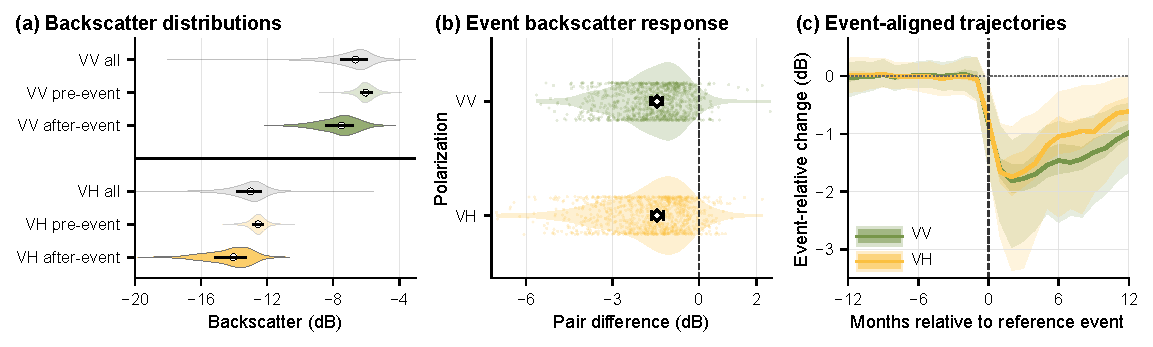
\includegraphics[width=\linewidth]{figures/fig05_population_s1_signatures.pdf}
    \caption{Sentinel-1 signatures of balsa stand disturbances.
    (a) Absolute VV and VH distributions across all observations from the 3,498 polygons and within the pre-event ($-12$ to $-3$ months) and event/post-event (0 to $+2$ months) periods.
    (b) Paired event/post-minus-pre changes for 1,018 reference events; diamonds show medians and bars show 95\% complete-spatial-block bootstrap confidence intervals.
    (c) Event-aligned deviations from the pre-event background; dark and light ribbons show interquartile ranges and pointwise 95\% block-bootstrap confidence intervals, respectively.}
    \label{fig:s1_population_signatures}
\end{figure*}

Within-event changes were considerably more consistent than the absolute backscatter values. Across 1,018 reference events, median event/post-minus-pre change was $-1.46$~dB for VV (95\% spatial-block bootstrap CI, $-1.66$ to $-1.26$~dB) and $-1.45$~dB for VH ($-1.64$ to $-1.23$~dB), with negative changes in 96.4\% and 94.1\% of events, respectively (Fig.~\ref{fig:s1_population_signatures}b). Event-aligned median departures reached approximately $-1.8$~dB by month $+2$ and remained negative at month $+12$ ($-1.0$~dB for VV and $-0.6$~dB for VH); pointwise 95\% block-bootstrap intervals remained below zero throughout this period (Fig.~\ref{fig:s1_population_signatures}c). These results show that disturbance was more consistently expressed as a relative departure from the recent stand background than as an absolute backscatter state.

The representative stand showed the same temporal pattern (Fig.~\ref{fig:timeseries_signature}). The March 2024 reference disturbance coincided with coherent VV and VH declines and an optical transition from dense canopy to exposed ground, while earlier events in April 2019 and February 2022 illustrated repeated disturbance--recovery dynamics within the same stand. Similar absolute backscatter levels occurred during different stages of recovery and disturbance, further illustrating the value of interpreting change relative to the stand's recent temporal context.

% ---------------------------------------------------------------
\subsection{Sensitivity to stand representation, window geometry, and polarization}
\label{sec:representation_configuration}
% ---------------------------------------------------------------

Detection performance was generally stable across reasonable choices of stand representation, window geometry, and polarization, with no alternative providing a clear F1 improvement over the retained configuration (Fig.~\ref{fig:stand_representation_sensitivity}).

\begin{figure*}[pos=!htbp]
    \centering
    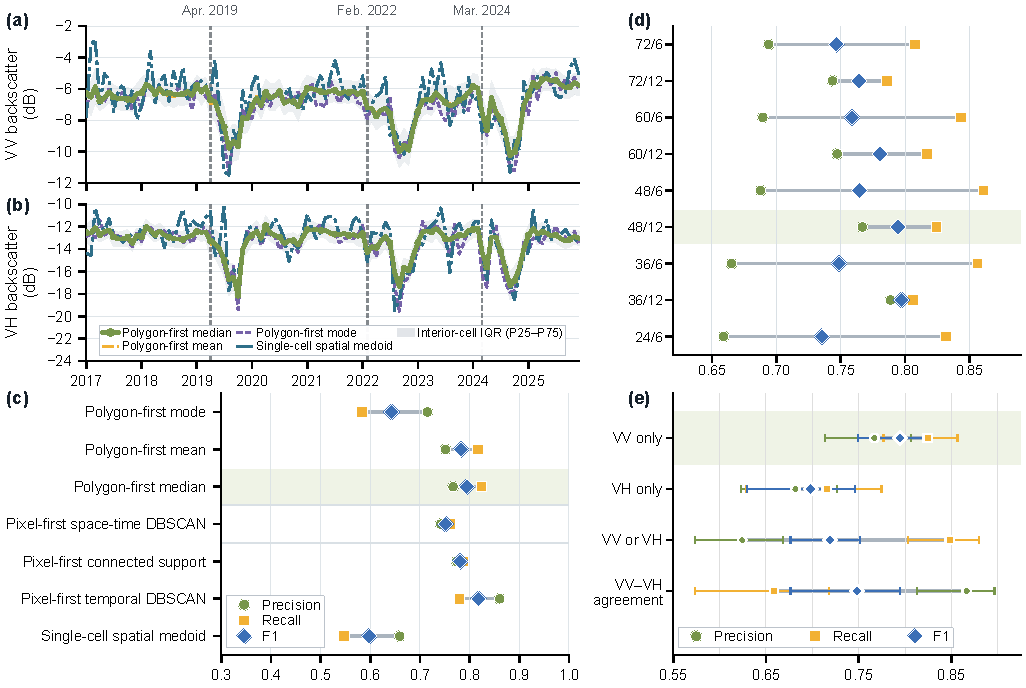
\includegraphics[width=\linewidth]{figures/fig07_representation_configuration.pdf}
    \caption{Sensitivity of Windowed CUSUM to stand representation, window geometry, and polarization.
    (a,b) Illustrative monthly VV and VH stand trajectories with within-polygon cell interquartile ranges and reference-event months.
    (c--e) Event-level precision, recall, and F1 across stand representations, window configurations, and polarization strategies.
    Connected support used the spatially selected threshold $r=0.20$; whiskers show 95\% spatial-block bootstrap confidence intervals, and highlighting indicates the retained configurations.}
    \label{fig:stand_representation_sensitivity}
\end{figure*}


Under the fixed 48-month window, 12-month displacement, and $p_{\mathrm{perm}}\leq0.025$ threshold, the Polygon-first median achieved precision 0.767, recall 0.824, and F1 0.795. The highest alternative point estimate was obtained by Pixel-first temporal DBSCAN (F1 = 0.818), but its paired F1 advantage was uncertain ($+0.024$, 95\% CI: $-0.005$ to 0.049). Connected support with the spatially selected $r=0.20$ achieved precision 0.774, recall 0.788, and F1 0.781, differing from the median by $-0.014$ (95\% CI: $-0.034$ to 0.007). The Polygon-first median was therefore retained because it provided a direct stand-level trajectory, high recall, and no additional support or clustering parameters.

Window geometry had similarly limited influence near the retained configuration. The highest fixed F1 was 0.797 for 36/12, only $+0.003$ above 48/12 (95\% CI: $-0.013$ to 0.019). Although 36/12 was selected in all five outer folds, its nested spatial out-of-fold performance remained essentially equivalent to the prospectively locked 48/12 configuration. The 48/12 geometry was therefore retained.

VV-only produced the highest F1 among the evaluated polarization strategies (precision 0.767, recall 0.824, F1 0.795). Accepting detections from either polarization increased recall at the expense of precision, whereas requiring VV--VH agreement increased precision but reduced recall. Neither strategy improved F1, and VV-only was retained for the final disturbance-history reconstruction.


% -----------------------------------------------------------
\subsection{Component attribution of Windowed CUSUM}
\label{sec:representation_component_ablation}
% -----------------------------------------------------------

Component analysis showed that local-reference windowing was the main source of recurrent-event sensitivity, while central-interval admission and permutation calibration progressively recovered precision (Table~\ref{tab:component_ablation}). Adding local-reference windows increased recall from 0.349 to 0.878 and F1 by $+0.137$ (95\% CI: 0.075--0.198), although precision decreased to 0.493. Central-interval admission increased precision to 0.684 and produced a further F1 gain of $+0.127$ (0.103--0.146). The negative-shift constraint had negligible incremental effect, whereas permutation-based calibration increased precision from 0.687 to 0.767 and F1 by $+0.036$ (0.022--0.049), yielding the complete detector F1 of 0.795.

\begin{table*}[pos=!htbp]
    \centering
    \small
    \caption{Progressive component attribution under the fixed 48/12 configuration. $\Delta F1$ compares each cumulative configuration with its predecessor; intervals are paired 95\% spatial-block bootstrap confidence intervals.}
    \label{tab:component_ablation}

    \begin{tabular}{lrrrrc}
        \toprule
        Cumulative configuration &
        Detections &
        Precision &
        Recall &
        F1 &
        Incremental $\Delta F1$ [95\% CI] \\
        \midrule
        Global CUSUM
        & 447
        & 0.852
        & 0.349
        & 0.495
        & -- \\

        + Local-reference windows
        & 1,948
        & 0.493
        & 0.878
        & 0.631
        & $+0.137$ [0.075, 0.198] \\

        + Central decision interval
        & 1,362
        & 0.684
        & 0.852
        & 0.758
        & $+0.127$ [0.103, 0.146] \\

        + Negative-shift constraint
        & 1,350
        & 0.687
        & 0.848
        & 0.759
        & $+0.000$ [$-0.003$, 0.003] \\

        + Permutation-based calibration
        & 1,175
        & 0.767
        & 0.824
        & \textbf{0.795}
        & $+0.036$ [0.022, 0.049] \\
        \bottomrule
    \end{tabular}
\end{table*}

Controlled-removal analysis supported the same ordering. Removing local-reference windowing reduced F1 by 0.327 (95\% CI: 0.280--0.370), compared with reductions of 0.038 for the central decision interval and 0.036 for permutation calibration; removing the negative-shift constraint again had negligible effect. Together, the two analyses indicate that recurrent-event sensitivity was driven primarily by repeated local-reference renewal, whereas central admission and local statistical calibration controlled the precision lost when additional candidate events became detectable. Because the Global CUSUM baseline can nominate only one candidate per trajectory, this contrast isolates component contributions within the ablation framework and is not a substitute for comparison with recurrent benchmark detectors.



% -----------------------------------------------------------
\subsection{Benchmark performance and statistical robustness}
\label{sec:benchmark_null_sensitivity}
% -----------------------------------------------------------

Under five-fold spatial out-of-fold evaluation, Windowed CUSUM achieved precision 0.789, recall 0.806, F1 0.797, and matched-event MAE 0.776 months (Table~\ref{tab:benchmark_comparison}). The highest benchmark F1 was 0.680 for CCDC, followed by 0.675 for decrease-filtered ReCuSum. Primary F1 differences were $+0.117$ against CCDC (97.5\% CI: 0.085--0.172) and $+0.454$ against monthly CuSum NRT (97.5\% CI: 0.412--0.491). ReCuSum attained similar precision to Windowed CUSUM (0.787 versus 0.789) but substantially lower recall (0.591 versus 0.806); the paired F1 difference was $+0.122$ (95\% CI: 0.094--0.149). Thus, the advantage over this recurrent detector arose primarily from improved event recall.

Exploratory CCDC expansion yielded F1 0.669 (change $-0.011$, 95\% CI: $-0.023$ to 0.005), without evidence of improvement. On 626 shared reference events, Windowed CUSUM had higher MAE than original CCDC (difference 0.101 months, 95\% CI: 0.014--0.205). The Windowed CUSUM advantage concerned detection balance, not uniformly higher recall or lower dating error.

\begin{table}[pos=!htbp]
    \centering
    \small
    \caption{Five-fold spatial out-of-fold benchmark using Polygon-first median VV trajectories and $\pm2$-month event matching. CCDC uses the original search; MAE includes matched events only.
    }
    \label{tab:benchmark_comparison}

    \begin{tabular}{lrrrr}
        \toprule
        Evaluated implementation & Precision & Recall & F1 & MAE (months) \\
        \midrule
        \textbf{Windowed CUSUM}
        & 0.789 & 0.806 & \textbf{0.797} & 0.776 \\

        CCDC 
        & 0.750 & 0.622 & 0.680 & 0.626 \\

        ReCuSum, decrease-filtered
        & 0.787 & 0.591 & 0.675 & 0.752 \\

        CuSum NRT, decrease-filtered
        & 0.414 & 0.844 & 0.556 & 0.875 \\

        BOCD prototype, decrease-filtered
        & 0.740 & 0.343 & 0.469 & 0.747 \\

        ReCuSum, raw
        & 0.419 & 0.513 & 0.461 & 0.743 \\

        Maximum monthly decline
        & 0.335 & 0.572 & 0.422 & 0.755 \\

        CuSum NRT, monthly adaptation
        & 0.222 & 0.754 & 0.344 & 0.898 \\

        Classical lower CUSUM
        & 0.171 & 0.290 & 0.215 & 1.498 \\
        \bottomrule
    \end{tabular}
\end{table}

The recall advantage over decrease-filtered ReCuSum was most pronounced in polygons with multiple recorded disturbances. For polygons containing one, two, and at least three reference events, Windowed CUSUM achieved recalls of 0.891, 0.813, and 0.794, compared with 0.764, 0.624, and 0.553 for ReCuSum. In the at-least-three-event group, the paired recall difference reached $+0.240$ (95\% CI: 0.179--0.289), consistent with the intended role of local-reference renewal in recurrent-event detection. These strata describe recorded reference-event multiplicity and are not assumed to represent complete disturbance histories.

Temporal-null formulation primarily shifted the precision--recall operating point. Under the fixed 48/12 configuration, finite-sample independent-value permutation yielded F1 0.795, compared with 0.791 for the archived empirical-rank implementation. A three-month calendar-block permutation increased precision to 0.828 but reduced recall to 0.676 and F1 to 0.745 ($\Delta F1=-0.050$, 95\% CI: $-0.084$ to $-0.028$). Six-month blocks further reduced recall to 0.339, while 12-month blocks admitted no events at the common threshold. Moving-block-bootstrap nulls yielded F1 values of 0.667--0.725, and the track-wise maximum-statistic null yielded 0.365. Monte Carlo seed variation was negligible relative to differences among null formulations. The independent-value permutation therefore provided the highest F1 under the common threshold, although this comparison demonstrates sensitivity to null assumptions rather than establishing its statistical calibration as uniquely correct.


% 需要多少 post-event evidence 才能稳定检测？冻结后的方法在真实 incomplete terminal record 上能否运行？
% -----------------------------------------------------------
\subsection{Temporal truncation and prospective performance}
\label{sec:temporal_prospective_results}
% -----------------------------------------------------------

Temporal truncation showed that detection sensitivity increased as post-disturbance evidence accumulated. Among the 1,065 reference events evaluable at every horizon, recall increased from 0.202 using observations available only through the reference month to 0.613 after three months, 0.790 after six months, and 0.849 after 12 months. Event timing was comparatively stable once a detection had been established: of the 841 events detected by the six-month horizon, 814 (96.8\%) were assigned a month within $\pm2$ months of their corresponding 12-month estimate. Thus, limited post-event support primarily constrained whether an event was detected, rather than the stability of its estimated timing once sufficient evidence had accumulated.

A prospective replay of the locked detector using observations available through June 2026 produced 139 provisional disturbance candidates. Manual review was conducted for 95 sampled candidate polygons. After accounting for the prespecified sampling fractions, 57.5\% of candidates were estimated to represent confirmed disturbances (95\% spatial-block bootstrap CI: 0.287--0.812), increasing to 64.0\% (95\% CI: 0.393--0.846) when probable disturbances were included. Because validation was conditioned on detector-generated candidates, these estimates characterize candidate precision and prospective behaviour, but do not quantify missed disturbances or population recall.

% -----------------------------------------------------------------------
% -----------------------------------------------------------------------
\subsection{Recurrent disturbance histories and rotation-relevant intervals}
\label{sec:rotation_dynamics}
% -----------------------------------------------------------------------

Application of the locked VV-only Windowed CUSUM to the 3,498 validated balsa polygons identified 6,658 disturbance events during 2017--2025 (Fig.~\ref{fig:national_recurrence_patterns}). Event recurrence showed marked spatial heterogeneity, and annual detections ranged from 308 in 2023 to 1,026 in 2022. 
% Across the inventory, 82.9\% of polygons contained one to three detected events, whereas 349 contained none.

Among the 2,194 polygons with at least two detections, consecutive events defined 3,509 inter-disturbance intervals. The median interval was 36 months (IQR: 22--46 months; 95\% spatial-block bootstrap CI: 35--38 months), and 53.0\% of intervals fell between 24 and 47 months (Fig.~\ref{fig:national_recurrence_patterns}d). Short intervals were also common, with 20.4\% shorter than 12 months, indicating that successive detections cannot all be interpreted as complete plantation rotations.

Cross-polarization analysis tested whether the approximately three-year recurrence was specific to the VV-derived event sequence. Requiring both bounding VV events to have a one-to-one VH match within $\pm2$ months retained 1,385 intervals from 1,081 polygons, representing 39.5\% of all VV intervals (Fig.~\ref{fig:polarization_interval_sensitivity}). Their median was 40 months (IQR: 34--48 months; 95\% CI: 38--41 months), four months longer than the full VV estimate (paired 95\% CI: $+2$ to $+5$ months). VH support was less frequent for short intervals, indicating preferential retention of longer intervals rather than an unbiased correction of the VV distribution. Nevertheless, the dominant approximately three-year recurrence remained evident under cross-polarization support.

These intervals describe recurrent stand turnover observed within the Sentinel-1 record rather than independently verified planting-to-harvest cycles. The 36-month median is therefore interpreted as a rotation-relevant recurrence timescale, while individual disturbance events and short intervals require additional evidence before attribution to harvesting or complete biological rotations.

\begin{figure*}[pos=!htbp]
    \centering
    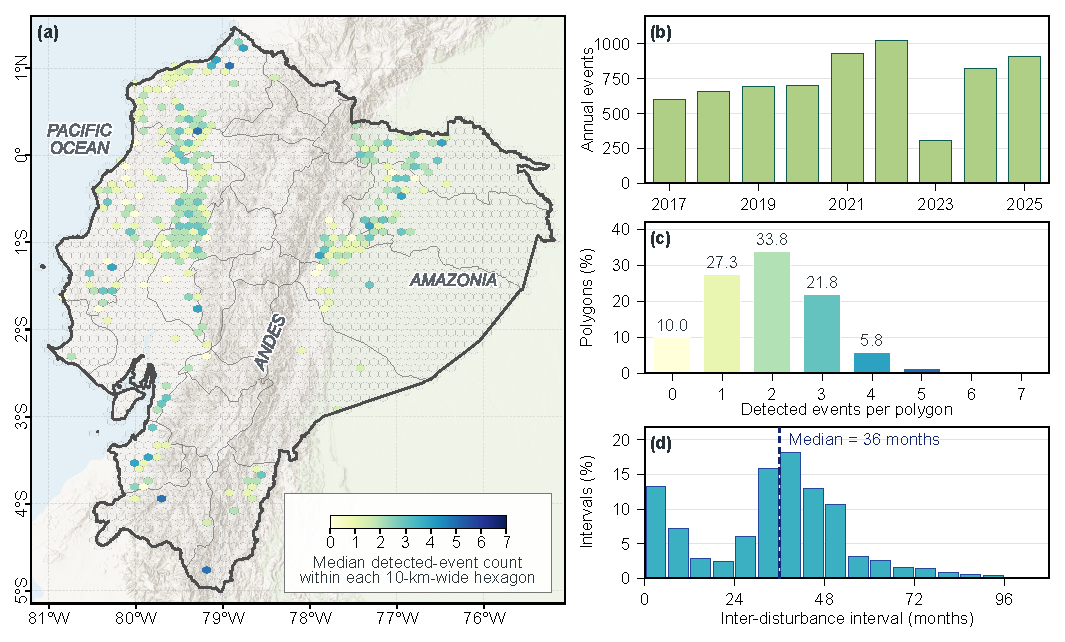
\includegraphics[width=\linewidth]{figures/fig01_national_recurrence.pdf}

    \caption{Reconstructed recurrent disturbances across the Ecuadorian balsa inventory.
    (a) Median detected-event count within fixed 10-km-wide hexagons.
    (b) Annual counts of the 6,658 detected events during 2017--2025.
    (c) Event-count distribution.
    (d) Distribution of 3,509 consecutive inter-disturbance intervals.}

    \label{fig:national_recurrence_patterns}
\end{figure*}

\begin{figure*}[pos=!htbp]
    \centering
    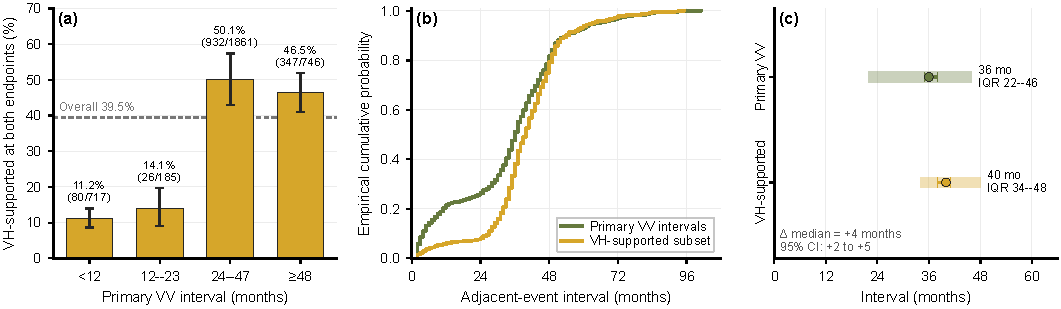
\includegraphics[width=\linewidth]{figures/fig08_polarization_intervals.pdf}

    \caption{Cross-polarization sensitivity of observed inter-disturbance intervals.
    (a) Fraction of VV-defined intervals for which both bounding events had corresponding VH detections within $\pm2$ months.
    (b) Empirical cumulative distributions of all VV intervals ($n=3{,}509$) and the VH-supported subset ($n=1{,}385$).
    (c) Median and interquartile interval estimates with 95\% spatial-block bootstrap confidence intervals.}

    \label{fig:polarization_interval_sensitivity}
\end{figure*}

% !TeX root = ../main.tex
% ============================================================
\section{Discussion}
\label{sec:discussion}
% ============================================================


% ------------------------------------------------------------
\subsection{Geometry-consistent trajectories and dual local adaptation}
% ------------------------------------------------------------

The central methodological result is that recurrent disturbance evidence was more consistently expressed relative to the recent state and variability of each stand than by absolute Sentinel-1 backscatter alone. Absolute VV and VH distributions overlapped substantially, whereas historical disturbances showed highly repeatable within-stand declines. This distinction motivates the three linked elements of the framework: acquisition geometry is kept consistent within each track-specific trajectory, overlapping windows repeatedly renew the local temporal reference, and a window-specific permutation null calibrates each CUSUM amplitude against the variability of that same local context.

Keeping Sentinel-1 tracks separate is important because systematic differences among acquisition geometries would otherwise enter the temporal background against which disturbance is evaluated. Track separation does not eliminate moisture, phenological, or structural variability, but it provides an internally comparable observation sequence within which local adaptation can operate. Windowed CUSUM then addresses the remaining temporal heterogeneity at two levels. Local-reference renewal allows later disturbances to be evaluated against the evolving stand condition, while local statistical calibration means that the same raw CUSUM amplitude need not represent the same level of evidence in a stable and a highly variable trajectory.

The component analysis supports this interpretation. Local-reference windowing produced the largest gain in recurrent-event sensitivity, whereas central-interval admission and permutation calibration progressively recovered precision. The benchmark results showed the same pattern: compared with decrease-filtered ReCuSum, Windowed CUSUM retained similar precision but substantially higher recall, particularly in polygons containing multiple recorded disturbances. The methodological contribution is therefore not windowing alone. CuSum NRT already applies CUSUM to short sliding time series for near-real-time monitoring~\citep{Ygorra2024CuSumNRT}, while ReCuSum handles repeated changes through recursive segmentation~\citep{Ygorra2023ReCuSum}. Here, overlapping local contexts, central event admission, and window-specific statistical calibration are coupled to reconstruct repeated events along a long stand trajectory without making later detections conditional on earlier segmentation.

These comparisons refer to the evaluated stand-level adaptations and should not be interpreted as demonstrating superiority over the complete operational CuSum NRT, CCDC, or published polarimetric BOCD systems.


% ------------------------------------------------------------
\subsection{Recurrent disturbance histories and rotation-relevant interpretation}
% ------------------------------------------------------------

The methodological framework enabled individual detections to be translated into recurrent stand histories. Across the monitored balsa inventory, consecutive detected disturbances showed a dominant approximately three-year timescale, with a median interval of 36 months. This central tendency is consistent with the rapid growth and short commercial development periods reported for balsa in Ecuador~\citep{GonzalezOsorio2010Balsa,CanadasLopez2019BalsaGrowth}, but it should not be interpreted as a directly observed planting-to-harvest age.

% The resulting subset is therefore a robustness check rather than a corrected rotation estimate.
Cross-polarization analysis supports the persistence of this recurrence pattern while also illustrating its uncertainty. Requiring VH support at both bounding events retained a subset with a median interval of 40 months, but VH agreement preferentially retained longer intervals. More generally, balsa rotation length is expected to vary with site productivity, management, and market conditions, and longer commercial cycles have been reported in other production systems~\citep{Jenkin2019BalsaValueChain,Midgley2010Balsa}.

Several features of the detected histories further limit a direct biological interpretation. Planting dates were unavailable, the first and last cycles were censored by the observation period, omitted disturbances can lengthen observed intervals, and additional detections can shorten them. The presence of intervals below 12 months also indicates that not every pair of successive negative transitions corresponds to a complete harvest--regrowth cycle. Individual detections may represent clear-cutting, partial removal, repeated clearing, or other structural changes. The 36-month estimate is therefore best interpreted as a rotation-relevant recurrence timescale of observed stand turnover within the Sentinel-1 record.

The value of the near-decadal archive lies in this ability to observe repeated transitions within the same management units. Longer temporal coverage increases the number of complete adjacent-event intervals that can be reconstructed, extending SAR monitoring beyond isolated disturbance alerts toward multi-cycle plantation histories.


% ------------------------------------------------------------
\subsection{Robustness, limitations, and transferability}
% ------------------------------------------------------------

The evaluation design addressed several sources of optimistic performance estimation but does not eliminate all uncertainty. Spatial blocking kept geographically related polygons, tracks, and events together during parameter selection and evaluation, reducing spatial leakage~\citep{Roberts2017SpatialCV}. However, performance remains conditional on the available reference catalogue and does not constitute independent geographic validation. Unrecorded disturbances can reduce apparent precision, while reference dates partly derived from remote-sensing interpretation may retain some sensor-related dependence.

Statistical calibration is another important boundary. The independent-value permutation provided the highest F1 among the evaluated null formulations at the common threshold, but dependence-preserving alternatives shifted the detector toward higher precision and substantially lower recall. This result should not be interpreted as proof that monthly Sentinel-1 observations are exchangeable. Rather, the retained permutation null represents an empirically effective operating choice under the evaluated precision--recall trade-off. Stronger statistical error-control claims would require independently observed no-disturbance periods, explicit null simulations, or dependence-aware resampling schemes that preserve realistic short-range temporal structure~\citep{Kunsch1989BlockBootstrap}.

Temporal truncation also distinguishes retrospective event reconstruction from immediate alerting. Recall increased substantially as post-disturbance observations accumulated, reaching 0.790 after six months, while 96.8\% of events already detected at that horizon were dated within two months of their corresponding 12-month estimates. Thus, limited post-event support primarily affected whether a disturbance accumulated sufficient evidence for detection, rather than the stability of its estimated month once detected. Monthly compositing further means that estimated event months should not be interpreted as exact felling dates.

Disturbance attribution remains a separate limitation. Negative Sentinel-1 transitions can be associated with harvesting but may also arise from partial canopy removal, flooding, storm damage, or other surface-state changes, and apparent performance depends on reference design and disturbance definition~\citep{RodriguezPaulino2024Review}. The prospective 2026 review was candidate-conditioned and therefore informs candidate precision but cannot estimate missed disturbances or population recall.

The transferable contribution is consequently not a fixed balsa-specific threshold, but a framework in which observation geometry is controlled before detection and both temporal background and statistical evidence are adapted locally. This structure is potentially applicable to other short-rotation plantation systems with repeated management disturbances and limited optical continuity. Future work should determine when provisional candidates have accumulated sufficient post-disturbance evidence to be considered temporally stable and develop dependence-aware statistical calibration that preserves realistic Sentinel-1 temporal structure without the substantial recall loss observed under conservative block-based nulls.
% !TeX root = ../main.tex

\section{Conclusion}

Windowed CUSUM provides a locally adaptive framework for reconstructing recurrent stand disturbances from long Sentinel-1 time series. Track-specific trajectories preserve acquisition-geometry consistency, overlapping windows repeatedly renew the temporal reference, and window-specific permutation calibration evaluates each CUSUM departure relative to the variability of the same local context. Under spatial out-of-fold evaluation, Windowed CUSUM achieved an F1 of 0.797, compared with 0.680 for CCDC VV and 0.675 for decrease-filtered ReCuSum. The advantage arose primarily from higher recurrent-event recall. Component analysis further identified local-reference renewal as the main source of sensitivity, while central event admission and local statistical calibration recovered precision.

Applied to 3,498 validated balsa polygons, the locked detector reconstructed 6,658 disturbances and 3,509 consecutive inter-disturbance intervals during 2017--2025, with a median recurrence of 36 months. More broadly, the study shows that geometry-consistent SAR trajectories combined with local temporal and statistical adaptation can extend disturbance monitoring from isolated change detection toward reconstruction of recurrent plantation disturbance histories in cloud-prone regions.
% !TeX root = ../main.tex
\section*{Data and code availability}
The accompanying repository contains the Windowed CUSUM source, frozen configuration, aggregate results and provenance manifests. The radar source is the NASA OPERA RTC-S1 archive~\citep{opera2023rtc}; S1-GRiTS provides its catalogue and cube organization. Exact plantation geometries, dated references and pixel caches require review of redistribution rights and location-disclosure conditions. Planet imagery and third-party basemap caches are not included in the public release. A verified public repository URL and archival identifier remain to be assigned before submission; no permanent identifier is asserted in this draft.

\section*{Ethics declaration}
The study used satellite observations, administrative plantation polygons and historical stand-event records. It did not involve human participants, personal data or animal experiments.

\section*{Conflict of interest}
The authors declare that they have no known competing financial interests or personal relationships that could have influenced the work reported in this article.

\section*{Funding}
This work was supported by the Startup Research Fund of Henan Academy of Sciences (No.~242025005) and the Open Research Fund Program of the MNR Key Laboratory for Geo-Environmental Monitoring of the Great Bay Area.

\section*{Declaration of generative AI and AI-assisted technologies}
OpenAI Codex was used to assist with repository auditing, reproducible analyses, literature-metadata checking and English-language drafting. The authors are responsible for reviewing and verifying the manuscript, its numerical results and its citations before submission, and for the content of the submitted article.


\printcredits
\bibliographystyle{cas-model2-names}
\bibliography{references}

\end{document}
